\chapter{�bungsbl�tter}
\section{�bungsblatt 01}
\subsection{Aufgabe 1.1}
\subsubsection{L�sung}
\renewcommand{\labelenumi}{\alph{enumi})}
\begin{enumerate}
\item zu zeigen $(A \triangle B) \backslash C = (A \backslash C) \triangle (B \backslash C)$\\
		Analytischer Beweis
		\begin{alignat*}{2}
			LS &= (A \triangle B) \backslash C\\
			&= ((A \ohne B) \cup (B \ohne A)) \ohne C\\
			&= ((A \ohne B) \cup (B \ohne A)) \cap \overline{C}\\
			&= ((A \cap \overline{B}) \cup (B \cap \overline{A})) \cap \overline{C}\\
			&= ((A \cap \overline{B}) \cap \overline{C}) \cup ((B \cap \overline{A}) \cap \overline{C})
		\end{alignat*}
		\begin{alignat*}{2}
			RS &= (A \ohne C) \triangle (B \ohne C)\\
			&= (A \cap \overline{C}) \triangle (B \cap \overline{C})\\
			&= ((A \cap \overline{C}) \ohne (B \cap \overline{C}) \cup ((B \cap \overline{C}) \cap \overline{(A \cap \overline{C})})\\
			&\vdots\\
			&=(A \cap \overline{B} \cap \overline{C}) \cup (\overline{A} \cap B \cap \overline{C})
		\end{alignat*}
		Kern Diagramm\\
		%IMG-02.11.2008-mathe-1
		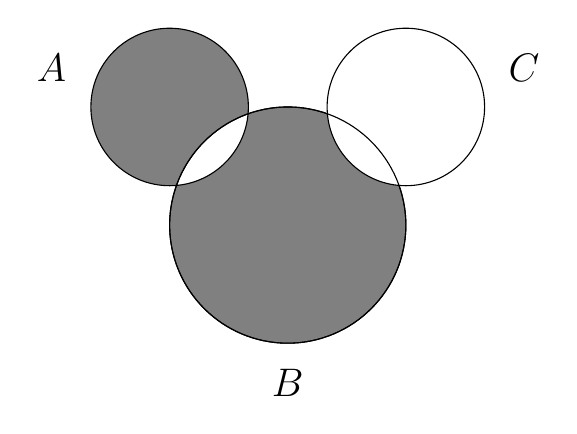
\begin{tikzpicture}
		\filldraw[fill=gray, even odd rule] (0,0) circle (1.5cm) (-1.5,1.5) circle (1cm);
		\filldraw[fill=white] (1.5,1.5) circle (1cm);
		\draw (0,0) circle (1.5cm);

		\node at (-3,2) {\Large{$A$}};
		\node at (0,-2) {\Large{$B$}};
		\node at (3,2) {\Large{$C$}};
		\end{tikzpicture}
\item zu zeigen $A \cap C = \emptyset \Ra (A \triangle B) \ohne C = A \triangle (B \ohne C)$\\
		Analytischer Beweis
		\[A \cap C = \emptyset \Ra A \ohne C = A\]
		\[(A \triangle B) \ohne C = (A \ohne C) \triangle (B \ohne C) = A \triangle (B \ohne C)\]
\end{enumerate}
\renewcommand{\labelenumi}{\arabic{enumi}.}

\subsection{Aufgabe 1.5}
$q_0 = 0$\\
$q_n = q_{n+1} + 2n - 1 \mbox{ f�r } n \in \mathbb{N}$\\
\textalign{Behauptung:}{$q_n = n^2 \mbox{ f�r alle } n \in \mathbb{N}$}
\textalign{Beweis:}{$ $\newline
$\left.\hspace{-0.7em}\begin{array}{ll}
(IA) n = 1&LS = q_1 = q_0 + 2 1 - 1 = 0 + 2 - 1 = 1\\
&RS = 1^2 = 1
\end{array}\right\} \checkmark$\\
$(IS) \mbox{ zu zeigen } \overbrace{q_n = n^2}^{(IV)} \Rightarrow q_{n+1} = (n + 1)^2\\
q_{n+1} = q_n + 2 (n + 1) - 1\\ %TODO align an zu zeigen
= n^2 + 2n + 1 = (n + 1)^2$}

\subsection{Aufgabe 1.6}
$0 \leq a_i < 1 \mbox{ f�r } i \in \mathbb{R}$\\
\textalign{Behauptung:}{$\forall n \in \mathbb{N} \prod_{i = 1}^n (1 - a_i) \geq 1 - \sum_{i = 1}^n a_i$}
\textalign{Beweis:}{$ $\newline
$\left.\hspace{-0.7em}\begin{array}{ll}
(IA) n = 1 & LS = \prod_{i = 1}^1 (1 - a_i) = (1 - a_1)\\
&RS = 1 - \sum_{i = 1}^1 a_i = 1 - a_1
\end{array}\right\} \checkmark$\\
$(IS) \mbox{ zu zeigen } \overbrace{\prod_{i = 1}^n (a - a_i) \geq 1 - \sum_{i = 1}^n a_i}^{(IV)} \Rightarrow \prod_{i = 1}^{n + 1} a_i\\
\prod_{i = 1}^{n + 1} (1 - a_i) = (1 - a_{n + 1}) \mal \prod_{i = 1}^n (1 - a_i)\\ %TODO align an "zu zeigen"
\geq (1 - a_{n + 1}) \mal (1 - \sum_{i = 1}^n a_i) = 1 - \sum_{i = 1}^n a_i - a_{n + 1} + a_{n + 1} \mal \sum_{i = 1}^n a_i\\
= 1 - \sum_{i = 1}^{n + 1} a_i + \underbrace{a_{n + 1} \mal \sum_{i = 1}^n a_i}_{\geq 0} \geq 1 - \sum_{i = 1}^{n + 1} a_i$}
\subsection{Aufgabe 1.7}
Behauptung:
%IMG-05.11.2008-mathe-1
\begin{tikzpicture}
	\draw (0,0) rectangle (2,2);

	\node at (1,2.3) {$2^n$};
	\node at (2.3,1) {$2^n$};
\end{tikzpicture} �berdeckbar mit
%IMG-05.11.2008-mathe-2
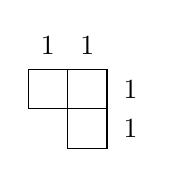
\begin{tikzpicture}
	\draw (0,0) rectangle (0.5,0.5);
	\draw (0.5,0) rectangle (1,0.5);
	\draw (0.5,0) rectangle (1,-0.5);

	\node at (0.25,0.8) {$1$};
	\node at (0.75,0.8) {$1$};
	\node at (1.3,0.25) {$1$};
	\node at (1.3,-0.25) {$1$};
\end{tikzpicture} f�r $n \in \mathbb{N}$
\renewcommand{\labelenumi}{Schritt \arabic{enumi}}
\begin{enumerate}
\item zu zeigen\\ IMGmathezwei �berdeckbar mit IMGmatheeins $n \in \mathbb{N}$
		\begin{align*}
			(IA) &n = 1~~\begin{minipage}{5mm} IMGmatheeins \end{minipage}\\
			&2^0 = 1
		\end{align*}
		\begin{align*}
			(IS) &\mbox{zu zeigen} \forall n \in \mathbb{N} IMGmathezwei \mbox{ �berdeckbar mit } IMG-05.11.2008-mathe-2\\
			&\Ra IMG-05.11.2008-mathe-3 \mbox{ �berdeckbar mit} IMG-05.11.2008-mathe-2\\
			&IMG-05.11.2008-mathe-4 \mbox{ die 4 } IMG-05.11.2008-mathe-5 \mbox{ der Gr��e $2^{n - 1}$ lassen sich nach $(IV)$ durch } IMG-05.11.2008-mathe-2 \mbox{ �berdecken}
		\end{align*}
\item Quadrat $d$ Seitenl�nge $2^n$ ohne ein IMG-05.11.2008-mathe-6 Feldchen l�sst sich mit IMG-05.11.2008-mathe-5 �berdecken\\
		\begin{align*}
			(IA) &n = 1 IMG-05.11.2008-mathe-7 \checkmark\\
			(IS) ~&\mbox{zu zeigen} \forall n \in \mathbb{N} \mbox{ ist Quadrat mit Seitenl�nge $2^n$}\\
			&\Ra \mbox{Quadrat mit Seiten $2^{n+1}$ ist in } IMG-05.11.2008-mathe-2 \mbox{ zerlegbar}\\
			&IMG-05.11.2008-mathe-8 IMG-05.11.2008-mathe-9 \mbox{nach Schritt 1 �berdeckbar}\\
			&IMG-05.11.2008-mathe-10 \mbox{nach $(IV)$ �berdeckbar}
		\end{align*}
\end{enumerate}
\renewcommand{\labelenumi}{\arabic{enumi}.}
\begin{flushright}$\blacksquare$\end{flushright}